%% Nature-style manuscript — Springer Nature template (sn-jnl, sn-nature style)
%% Compile: tectonic main.tex   (or pdflatex + bibtex)
\documentclass[pdflatex,sn-nature]{sn-jnl}

\usepackage{graphicx}
\usepackage{amsmath,amssymb,amsfonts}
\usepackage{booktabs}
\usepackage[title]{appendix}
\usepackage{xcolor}

\raggedbottom

\begin{document}

\title[Self-supervised ENSO-linked temperature regimes in Amazonia]{Self-supervised learning identifies statistically robust ENSO-linked temperature regimes in Amazonia}

\author*[1]{\fnm{L\'ivia} \sur{Meinhardt}}\email{livia.meinhardt@fgv.edu.br}
\author[1]{\fnm{D\'ario} \sur{Oliveira}}\email{dario.oliveira@fgv.br}

\affil*[1]{\orgdiv{School of Applied Mathematics (EMAp)}, \orgname{Funda\c{c}\~ao Getulio Vargas}, \orgaddress{\city{Rio de Janeiro}, \country{Brazil}}}

\abstract{The El Ni\~no--Southern Oscillation (ENSO) is the dominant driver of interannual climate variability in Amazonia, yet linking it to regional conditions typically relies on hand-crafted indices or grid-point regressions that ignore the spatial coherence of the response. Here we learn a compact vocabulary of daily temperature-anomaly regimes for Amazonia directly from data, by training a Masked Siamese Network with a Vision Transformer backbone on deseasonalised ERA5 daily minimum and maximum temperature fields (1981--2025) and discretizing the learned representation into fifteen prototypes. The regimes are spatially coherent, nearly season-independent, and reproduce warm and cool conditions consistently in every calendar month. Because the effective replication unit is the ENSO episode (35 in the record) rather than the $\sim$16{,}000 days, we evaluate teleconnections with an episode-aware statistical framework: an autocorrelation-preserving null, family-wise error control, block-bootstrap confidence intervals and split-half replication. A global test confirms that ENSO modulates regime occupancy ($P = 0.013$), and three regimes survive every gate: two El Ni\~no-like warm-anomaly regimes and one La Ni\~na-like cool-anomaly regime, whose spatial patterns independently match the composite ENSO fingerprint. The strongest regime occupies 19.7\% of El Ni\~no months versus 2.5\% of La Ni\~na months and its frequency has grown by 5.3 percentage points per decade, indicating that ENSO-linked warm-anomaly states are becoming more common. Self-supervised discretization thus provides an interpretable, statistically honest bridge between large-scale climate drivers and regional variability.}

\keywords{self-supervised learning, climate regimes, ENSO, teleconnections, Amazonia}

\maketitle

\section{Main}\label{sec:main}

The El Ni\~no--Southern Oscillation (ENSO) reorganizes atmospheric circulation across the tropics and is the leading source of interannual climate variability over South America\cite{ropelewski1987global,cai2020enso}. In Amazonia, El Ni\~no events have been associated with record-breaking warming, drought and fire risk\cite{jimenez2016record,marengo2016amazon}, with consequences that propagate to agriculture\cite{Luiz_Silva_2024}, the agricultural frontier\cite{Marengo2022} and public health\cite{tian2025dengue}. Characterizing how this large-scale driver expresses itself in regional daily conditions is therefore both scientifically and societally relevant.

A central obstacle is representation. Daily gridded fields are high-dimensional, noisy and strongly autocorrelated, so teleconnection analyses usually compress them --- into scalar indices, empirical orthogonal functions, or grid-point regressions. An alternative with a long history in midlatitude dynamics is the notion of \emph{regimes}: a small set of recurrent, spatially coherent states whose occupancy statistics respond to external forcing\cite{michelangeli1995weather,hannachi2017regimes}. Regimes preserve spatial structure while reducing the daily record to a categorical sequence that is easy to interrogate. Classical regime detection, however, relies on linear decompositions and distance-based clustering in grid space, which struggle with the nonlinear, multiscale organization of tropical temperature fields.

Modern machine learning offers a different route. Deep networks now match or exceed physics-based systems in weather prediction\cite{GraphCast,Kochkov2024,bodnar2025aurora}, and self-supervised methods learn semantically organized representations without labels. Here we use a Masked Siamese Network (MSN)\cite{msn} with a Vision Transformer backbone\cite{vit_paper} to learn representations of daily Amazonian temperature fields, and we exploit a property of the MSN objective that makes it natural for regime discovery: representation learning and clustering are performed jointly, through a set of learnable prototypes\cite{caron2020swav} that discretize the latent space during training. Applied to deseasonalised ERA5\cite{hersbach2020era5} daily minimum and maximum temperature over Amazonia (1981--2025), the method yields fifteen temperature-anomaly regimes --- modes of variability relative to the local seasonal cycle.

A second obstacle is inference. The daily record contains $\sim$16{,}000 samples, but ENSO episodes --- the real unit of replication for teleconnection claims --- number only 35 in the study period (contiguous runs of a common phase label), of which 9 are El Ni\~no events. Day-level significance tests therefore overstate confidence by orders of magnitude, a pervasive problem in climate diagnostics\cite{wilks2016stippling}. We evaluate every ENSO effect at monthly resolution against an autocorrelation-preserving circular-rotation null\cite{ebisuzaki1997method}, control the family-wise error rate (FWER) across regimes and lags with max-statistic permutation, attach year-block bootstrap confidence intervals, and require split-half temporal replication.

This combination of learned regimes and episode-aware statistics yields three findings. First, the learned regimes are physically meaningful: spatially coherent, persistent beyond single days, nearly independent of the calendar, and consistently warm or cool in raw temperature in every month of the year. Second, ENSO robustly modulates regime occupancy: a global omnibus test is significant ($P = 0.013$), and three regimes pass all gates --- two El Ni\~no-like warm regimes and one La Ni\~na-like cool regime whose spatial anomaly patterns independently reproduce the composite ENSO fingerprint. Third, the regime-frequency record carries a warming signal: warm-anomaly regimes, including the most ENSO-sensitive one, have become substantially more frequent over the past four decades, while cool-anomaly regimes decline.

\section{Results}\label{sec:results}

\subsection{A vocabulary of temperature-anomaly regimes}\label{sec:vocab}

We trained the MSN encoder on daily ERA5 minimum and maximum 2-m temperature (T$_{\min}$, T$_{\max}$) fields over Amazonia (18$^\circ$S--5.5$^\circ$N, 74$^\circ$W--44$^\circ$W), deseasonalised into per-grid-cell, per-calendar-month standardized anomalies (Methods). Each of the 16{,}436 days in 1981--2025 is assigned to one of $K = 15$ learned prototypes, converting the continuous record into a categorical regime sequence.

Figure~\ref{fig:regimes} shows the mean anomaly composite of each regime, ordered from coolest to warmest. The vocabulary spans a smooth gradient from strong basin-wide cool anomalies (C14, C3) through weak or dipolar transitional states to strong warm anomalies (C0, C6), each with distinct spatial structure --- centred on the central basin (C6), tilted toward the northeast (C8), or contrasting the basin with the coastal southeast (C1). All fifteen prototypes are used, with occupancy between 5.6\% and 7.6\%, indicating that the discretization does not collapse onto a few dominant states.

Four properties establish the regimes as meaningful climate states rather than arbitrary partitions (Fig.~\ref{fig:characterization}). First, deseasonalisation worked as intended: the mean seasonal span of monthly occurrence frequency is only 7.3 percentage points, so regimes are available essentially year-round rather than being synonyms for calendar months. Second, regime occupancy is temporally coherent: mean residence times range from 1.5 to 3.4 days, with the warmest (C6, 3.4 d) and coolest (C14, 2.4 d; C3, 2.8 d) regimes the most persistent, and day-to-day transitions concentrate near the diagonal of the transition matrix (Extended Data Fig.~\ref{fig:ed_transitions}). Third, regime frequencies carry a coherent long-term signal: the three fastest-growing regimes are all warm-anomaly states (C6, $+5.25$ percentage points per decade; C1, $+2.71$; C0, $+2.39$), while the three fastest-declining are all cool-anomaly states (C14, $-4.11$; C3, $-3.11$; C10, $-2.45$), a regime-space expression of regional warming. Fourth, the regimes pass a seasonally fair raw-temperature check: reconstructing raw (non-deseasonalised) temperature and compositing departures from each calendar month's climatology, the warmest regimes are warmer than normal and the coolest regimes cooler than normal in \emph{every} month in which they occur (100\% sign consistency; e.g. C6: $+0.95$\,K in T$_{\min}$ and $+1.46$\,K in T$_{\max}$; C3: $-1.04$\,K and $-0.84$\,K; Extended Data Fig.~\ref{fig:ed_sanity}).

\subsection{An episode-aware test of the ENSO teleconnection}\label{sec:stats}

We aggregated the daily regime sequence into monthly occupancy frequencies (531 months between January 1981 and April 2025) and paired it with the Oceanic Ni\~no Index (ONI)\cite{noaa_oni_index}, which spans $-1.8$ to $+2.6$ in the period and defines 67 El Ni\~no months, 91 La Ni\~na months and 373 neutral months across 35 ENSO episodes (Methods).

Before inspecting individual regimes, a single omnibus test asks whether ONI relates to regime occupancy at all: the statistic $\sum_k \mathrm{corr}(f_k, \mathrm{ONI})^2 = 0.485$ is significant against the circular-rotation null ($P = 0.013$), licensing per-regime analysis.

Figure~\ref{fig:enso_stats}a shows the primary per-regime test: the correlation between monthly occupancy and the continuous, signed ONI, which uses both event magnitude and the La Ni\~na half of the gradient. Eight of fifteen regimes are nominally significant ($P < 0.05$, versus $\sim$0.8 expected by chance), but only three survive family-wise correction across the fifteen tests: C6 ($r = 0.38$, 95\% CI 0.25--0.51, $P_{\mathrm{FWER}} = 0.011$), C0 ($r = 0.28$, CI 0.19--0.37, $P_{\mathrm{FWER}} = 0.022$) and C3 ($r = -0.25$, CI $-0.34$ to $-0.15$, $P_{\mathrm{FWER}} = 0.029$).

The familiar binary composite view --- the excess probability of each regime during El Ni\~no months (Fig.~\ref{fig:enso_stats}b) --- tells the same story with visibly less power: C6 gains $+11.1$ percentage points of occupancy during El Ni\~no, but the year-block bootstrap interval ($-0.5$ to $+25.1$) grazes zero, illustrating why we treat the continuous-ONI test as primary and the binary anomaly as descriptive.

Two robustness analyses complete the picture. The lagged cross-correlation map over $\pm$12 months (Fig.~\ref{fig:enso_stats}c) shows the physically expected smooth lag structure, but after family-wise correction across all $15 \times 25$ regime--lag cells only one cell survives; with this record length the teleconnection is statistically resolvable only as a contemporaneous signal, and apparent precursor or delayed responses should not be over-interpreted. Split-half replication (Fig.~\ref{fig:enso_stats}d) computes each regime's ONI correlation independently on 1981--2002 and 2003--2025: the per-regime correlations agree across halves ($r = 0.78$), and the three FWER-significant regimes lie in the correct quadrants in both halves, indicating a stationary sign of the effect rather than an artefact of a few strong events.

\subsection{El Ni\~no-like and La Ni\~na-like regimes match the ENSO fingerprint}\label{sec:physical}

The statistical gates select three regimes; their physical content is shown in Fig.~\ref{fig:physical}. C6, the most ENSO-sensitive regime, is a basin-wide warm anomaly peaking over the central Amazon, stronger in T$_{\min}$ than T$_{\max}$; C0 is a moderate warm anomaly with a distinct spatial emphasis along the northern basin and river corridors, stronger in T$_{\min}$; C3 is a basin-wide cool anomaly. For comparison, Fig.~\ref{fig:physical}b shows the model-independent ENSO fingerprint: the mean anomaly field of El Ni\~no minus La Ni\~na months.

The correspondence between the two is quantitative and was not imposed at any point of the pipeline. Projecting every regime composite onto the El Ni\~no composite (Fig.~\ref{fig:physical}c), the spatial correlation is positive for the positively ONI-correlated regimes (C6: $+0.44$; C0: $+0.34$) and negative for the negatively correlated regime (C3: $-0.33$); across all fifteen regimes the sign of the spatial similarity matches the sign of the temporal ONI correlation for every FWER-significant regime. The occupancy statistics behave accordingly (Fig.~\ref{fig:physical}d): C6 fills 19.7\% of El Ni\~no months but only 2.5\% of La Ni\~na months (7.9$\times$ contrast), C0 rises from 2.2\% under La Ni\~na to 10.6\% under El Ni\~no, and C3 shows the mirror-image preference (9.7\% under La Ni\~na versus 2.7\% under El Ni\~no). The 12-month rolling occupancy of the three regimes visibly co-moves with ONI throughout the record, including the 1997/98, 2015/16 and 2023/24 El Ni\~no events (Extended Data Fig.~\ref{fig:ed_timeseries}).

Notably, the ENSO-linked regimes are also the regimes with the strongest long-term trends (Section~\ref{sec:vocab}): the El Ni\~no-like warm regimes C6 and C0 are the first- and third-fastest-growing states, while the La Ni\~na-like cool regime C3 is among the fastest-declining. In regime space, regional warming manifests as the background climate drifting toward the configurations that El Ni\~no episodes transiently produce.

\section{Discussion}\label{sec:discussion}

Our results demonstrate that self-supervised discretization can recover a compact, physically interpretable regime description of Amazonian temperature variability, and that a small subset of these regimes carries a statistically robust ENSO signal. Three aspects of the analysis deserve emphasis.

First, deseasonalisation is not optional. ENSO events are phase-locked to the calendar (peaking in boreal winter), so any regime vocabulary that encodes the seasonal cycle will exhibit spurious ENSO associations through the shared seasonal confounder. Training on standardized anomalies removes this pathway: the resulting regimes are nearly season-independent (7.3\% mean seasonal span), and the ENSO signal that remains --- roughly twice as strong globally as in a seasonal-field variant of the model --- is attributable to interannual variability rather than to the annual cycle.

Second, honest inference changes the headline. At day-level resolution nearly every regime would appear overwhelmingly ENSO-significant; at episode-level resolution, with family-wise control, three of fifteen regimes survive. We regard this not as a weakness of the representation but as the honest ceiling of a 45-year, single-variable record containing 9 El Ni\~no episodes: the omnibus test is unambiguous, the surviving effects replicate across independent halves of the record, and their spatial patterns independently match the ENSO composite. The same discipline explains why we make no claims about lead--lag structure --- a 531-month series cannot support 375 simultaneous lag hypotheses --- even though the point estimates suggest the expected smooth lag evolution.

Third, the regime lens adds value beyond a confirmation of known teleconnections. It distinguishes two flavours of El Ni\~no-like warming (basin-centred C6 versus north-and-river-corridor C0) that a domain-mean index would merge; it localizes the La Ni\~na response in a specific cool configuration; and it reveals that the multi-decadal warming of Amazonia projects onto precisely the ENSO-linked regimes, connecting interannual and secular variability in a single description. Because the categorical sequence is cheap to condition on, it is directly usable downstream --- for compound-event analysis, as a covariate in impact models of fire, agriculture or vector-borne disease\cite{tian2025dengue,Luiz_Silva_2024}, or as a discrete state space for stochastic emulators.

The main limitations point to concrete extensions. Statistical power is bounded by episode count, and temperature is not the variable with the strongest Amazon ENSO response: adding precipitation --- with the methodological care its zero-inflated distribution requires --- and extending the record backward with ERA5's 1940--1980 segment would multiply both episodes and signal. Prototype identities are specific to a trained model (retraining permutes labels), so applications should track regime properties, not indices. Finally, the framework is region- and variable-agnostic: applying it to other climate modes, such as the Madden--Julian Oscillation or Atlantic variability, requires only a new bounding box and index.

\section{Methods}\label{sec:methods}

\subsection{Data}\label{sec:data}

We use hourly ERA5\cite{hersbach2020era5} minimum and maximum 2-m temperature (\texttt{mn2t}, \texttt{mx2t}) from January 1981 to December 2025, aggregated to daily minima and maxima respectively, on the native 0.25$^\circ$ grid over 18$^\circ$S--5.5$^\circ$N, 74$^\circ$W--44$^\circ$W ($94 \times 120$ grid cells). Each day is a tensor $x_t \in \mathbb{R}^{2 \times 94 \times 120}$. Years 2023--2025 are held out from encoder training as a validation split; regime assignments for the analysis are produced for all 16{,}436 days, and the ONI-matched monthly series covers January 1981 to April 2025 (531 months).

ENSO state is characterized by the Oceanic Ni\~no Index (ONI)\cite{noaa_oni_index,noaa_enso}, the three-month running mean of sea-surface-temperature anomalies in the Ni\~no~3.4 region. Following the operational definition, months belonging to runs of at least five consecutive overlapping seasons with ONI $> +0.5\,^\circ$C ($< -0.5\,^\circ$C) are labelled El Ni\~no (La Ni\~na); all others are neutral. Contiguous runs of a common label define episodes: the 531 analysis months contain 35 episodes, of which 9 are El Ni\~no, 8 La Ni\~na and 18 neutral.

\subsection{Deseasonalisation}\label{sec:deseason}

Because ENSO is phase-locked to the calendar, seasonal structure in the inputs would confound the teleconnection analysis. We therefore transform each grid cell to standardized anomalies: for cell $(i,j)$, variable $v$ and calendar month $m$, $\tilde{x}_{t,v,i,j} = (x_{t,v,i,j} - \mu_{v,i,j,m}) / \sigma_{v,i,j,m}$, with climatologies $\mu$ and $\sigma$ estimated from training years only to prevent leakage into the validation split. The resulting fields are approximately zero-mean and unit-variance by construction, and no further normalization is applied.

\subsection{Self-supervised regime learning}\label{sec:msn}

We formulate discretization as joint representation learning and clustering with a Masked Siamese Network\cite{msn}. Two Vision Transformer\cite{vit_paper} encoders are maintained: an anchor encoder $f_\theta$ trained by gradient descent and a target encoder $f_\xi$ whose weights are an exponential moving average of $\theta$. For each training day we generate one unmasked target view (random resized crop to $128 \times 128$) and eleven anchor views (one $128 \times 128$ random crop and ten $64 \times 64$ focal crops) with 15\% of anchor patches randomly dropped; random resized cropping is the sole augmentation, preserving physical values while varying spatial scale and coverage. Views are encoded and compared to $K = 15$ learnable prototypes $\{q_k\}$\cite{caron2020swav}: the assignment probability of representation $z$ is $p_k(z,\tau) \propto \exp(\langle z, q_k\rangle/\tau)$ with temperature $\tau = 0.1$, and target assignments are sharpened (0.25) with Sinkhorn--Knopp normalization. The loss is the cross-entropy between target and anchor assignments plus mean-entropy-maximization regularization, which enforces utilization of all prototypes and prevents collapse.

The backbone is a ViT-Small (patch size 16) modified for 2-channel input, with a 3-layer projection head (hidden 2048) to a 128-dimensional latent space. We train for 300 epochs with AdamW (batch 512; learning rate warm-up from $2\times10^{-4}$ to $10^{-3}$ over 15 epochs, cosine decay to $10^{-6}$; weight decay 0.04 increasing to 0.4) on a single NVIDIA A100.

At inference the anchor encoder is discarded. Each day is deterministically preprocessed (resize, centre crop to $128 \times 128$), encoded by $f_\xi$, and assigned to the prototype with maximal cosine similarity, yielding the categorical sequence used in all analyses.

\subsection{Episode-aware statistical framework}\label{sec:statsmethods}

All inference is performed on monthly regime frequencies $f_k(t)$ (the fraction of days of month $t$ in regime $k$), never on days, so that serial dependence and the episodic structure of ENSO enter the null distributions\cite{wilks2016stippling}.

\textbf{Null model.} Significance of any statistic is assessed against 5{,}000 circular rotations of the ONI series (or the El Ni\~no indicator) by a uniform random offset\cite{ebisuzaki1997method}. Rotation preserves the autocorrelation and episode-block structure of both series while destroying their alignment.

\textbf{Omnibus gate.} Before per-regime testing we compute $S = \sum_k \mathrm{corr}(f_k, \mathrm{ONI})^2$ and its rotation null. Per-regime results are interpreted only because this global test rejects ($S = 0.485$, $P = 0.013$).

\textbf{Per-regime tests and multiplicity.} The primary effect measure is the Pearson correlation between $f_k$ and the continuous, signed ONI. Family-wise error across the fifteen regimes is controlled by the max-statistic method: each rotation contributes its maximum absolute correlation across regimes, and $P_{\mathrm{FWER}}$ is the fraction of rotations whose maximum exceeds the observed value. The binary El Ni\~no anomaly $P(k \mid \text{El Ni\~no}) - P(k)$ is treated identically, rotating the El Ni\~no indicator. For the lag analysis, $\mathrm{corr}(f_k(t), \mathrm{ONI}(t-\ell))$ for $\ell \in [-12, 12]$ months, the max statistic is taken over all $15 \times 25$ regime--lag cells.

\textbf{Uncertainty.} 95\% confidence intervals for correlations and anomalies use a year-block bootstrap (2{,}000 resamples of whole calendar years with replacement), so that intra-annual dependence never inflates precision.

\textbf{Replication.} The record is split at its median year (2003) and per-regime ONI correlations are recomputed independently in each half; agreement is summarized by the correlation between the two vectors of per-regime effects.

\subsection{Composites, fingerprint and trends}\label{sec:composites}

Regime composites are the mean deseasonalised anomaly over training days assigned to the regime. The ENSO fingerprint is the mean anomaly over El Ni\~no months minus that over La Ni\~na months. Spatial similarity between a regime composite and the El Ni\~no composite is the centred spatial (Pearson) correlation over all cells and both variables. Long-term trends are ordinary-least-squares slopes of yearly mean occupancy versus year, expressed in percentage points per decade. The raw-temperature check reconstructs non-deseasonalised fields and composites the domain-mean departure from each calendar month's climatology, stratified by month to avoid re-exposing the seasonal cycle.

\subsection{Data availability}
ERA5 is available from the Copernicus Climate Data Store (\url{https://cds.climate.copernicus.eu}). The Oceanic Ni\~no Index is distributed by the NOAA Climate Prediction Center (\url{https://www.cpc.ncep.noaa.gov}).

\subsection{Code availability}
All code (training, inference, statistical framework and figure generation) is available at \url{https://github.com/Green-AI-Lab-GAIA/climate-clustering-for-ENSO-teleconnections}.

\backmatter

\bmhead{Acknowledgements}
This work was carried out at the School of Applied Mathematics, Funda\c{c}\~ao Getulio Vargas. Computations used an NVIDIA A100 GPU.

\bmhead{Author contributions}
L.M. designed the study, performed the experiments and analyses, and wrote the manuscript. D.O. supervised the research and revised the manuscript.

\bmhead{Competing interests}
The authors declare no competing interests.

%% ------------------------------------------------------------------ figures
\clearpage

\begin{figure}[p]
\centering
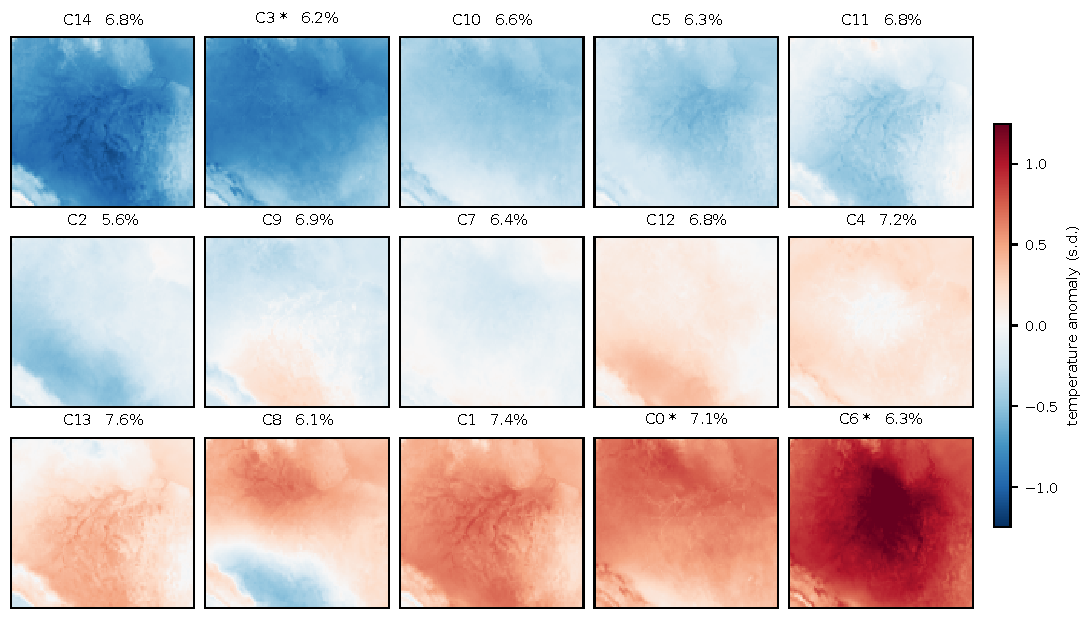
\includegraphics[width=\textwidth]{figures/fig1_regimes.pdf}
\caption{\textbf{Fifteen self-supervised temperature-anomaly regimes over Amazonia.}
Mean composite of the deseasonalised, per-cell standardized temperature anomaly (average of T$_{\min}$ and T$_{\max}$) for each learned regime, ordered from coolest (top left) to warmest (bottom right) mean anomaly. Panel titles give the regime label, its occupancy over 1981--2025, and an asterisk if the regime is FWER-significantly associated with ENSO (Fig.~\ref{fig:enso_stats}). Maps span 18$^\circ$S--5.5$^\circ$N, 74$^\circ$W--44$^\circ$W.}
\label{fig:regimes}
\end{figure}

\begin{figure}[p]
\centering
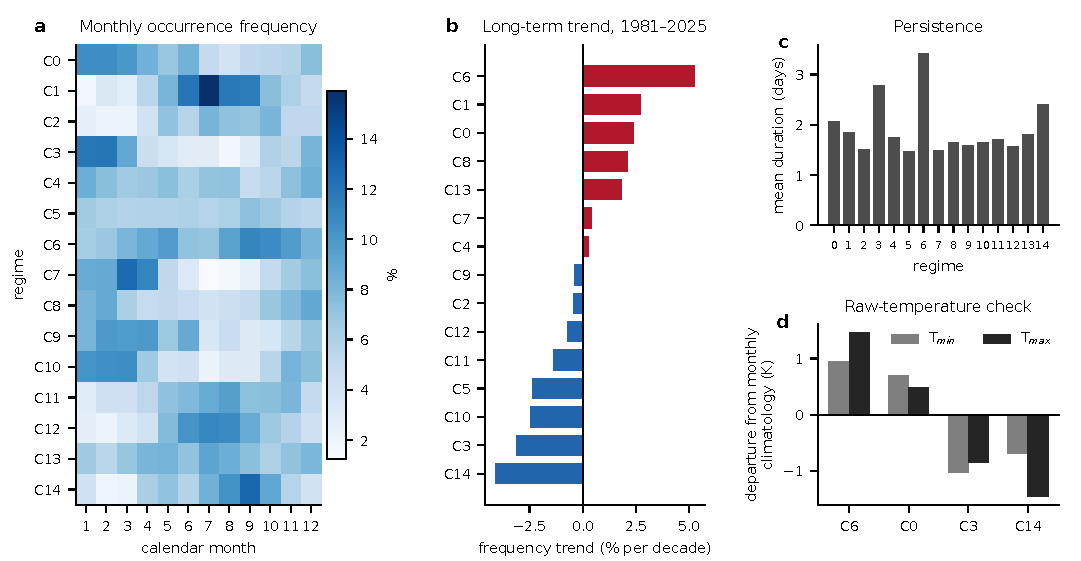
\includegraphics[width=\textwidth]{figures/fig2_characterization.pdf}
\caption{\textbf{The regimes are season-independent, persistent, trending and physically consistent.}
\textbf{a}, Mean monthly occurrence frequency of each regime; the mean seasonal span (maximum minus minimum across months) is 7.3 percentage points, confirming weak residual seasonality after deseasonalisation.
\textbf{b}, Long-term linear trend in yearly occupancy (percentage points per decade): the fastest-growing regimes are warm anomalies (red), the fastest-declining are cool anomalies (blue).
\textbf{c}, Mean residence time of each regime (consecutive-day runs).
\textbf{d}, Seasonally fair raw-temperature check for the two warmest (C6, C0) and two coolest (C3, C14) regimes: mean departure of domain-mean raw temperature from the corresponding calendar-month climatology. All four regimes keep the sign of their departure in 100\% of calendar months (Extended Data Fig.~\ref{fig:ed_sanity}).}
\label{fig:characterization}
\end{figure}

\begin{figure}[p]
\centering
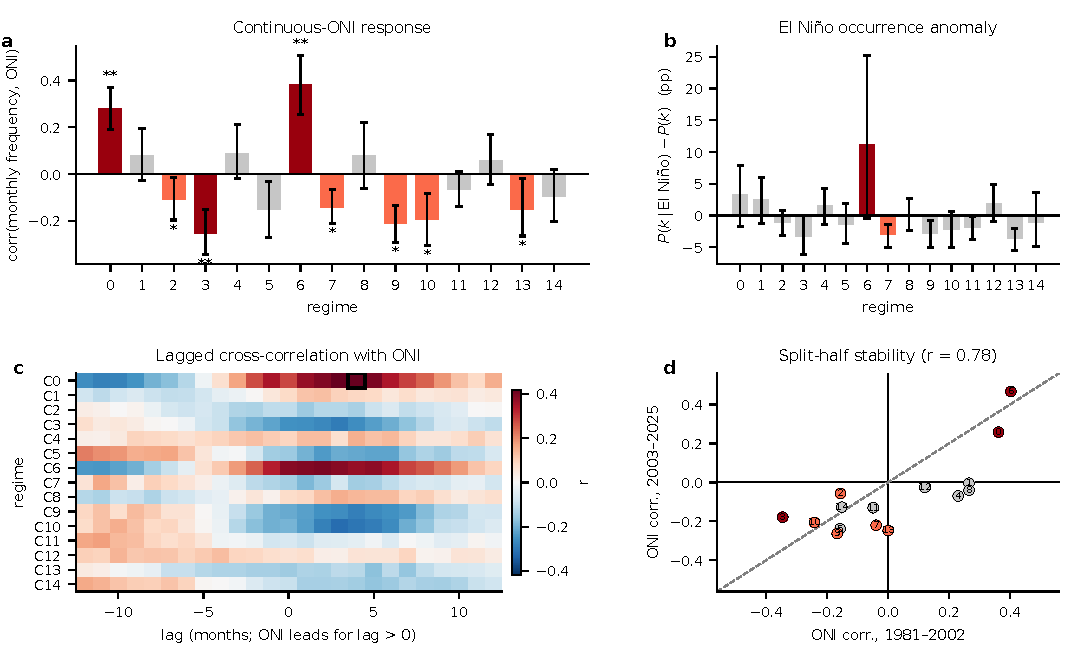
\includegraphics[width=\textwidth]{figures/fig3_enso_stats.pdf}
\caption{\textbf{Episode-aware significance of the ENSO--regime association} (531 months, 35 ENSO episodes; omnibus $P = 0.013$).
Throughout, dark red marks regimes significant after family-wise (FWER) max-statistic correction (also marked **), light red nominally significant only ($P<0.05$, *), grey not significant; error bars are 95\% year-block bootstrap confidence intervals.
\textbf{a}, Correlation between monthly regime frequency and the continuous, signed ONI --- the primary test. Three regimes survive FWER correction: C6 ($r=0.38$), C0 ($r=0.28$) and C3 ($r=-0.25$).
\textbf{b}, Binary El Ni\~no occurrence anomaly $P(k \mid \text{El Ni\~no}) - P(k)$ in percentage points --- the familiar composite view, shown with honest uncertainty.
\textbf{c}, Lagged cross-correlation between regime frequency and ONI; the black outline marks the only regime--lag cell (of 375) surviving FWER correction, so lead--lag structure is not statistically resolvable in this record.
\textbf{d}, Split-half replication: per-regime ONI correlations computed independently for 1981--2002 and 2003--2025 agree ($r = 0.78$), and all FWER-significant regimes fall in the correct quadrants in both halves.}
\label{fig:enso_stats}
\end{figure}

\begin{figure}[p]
\centering
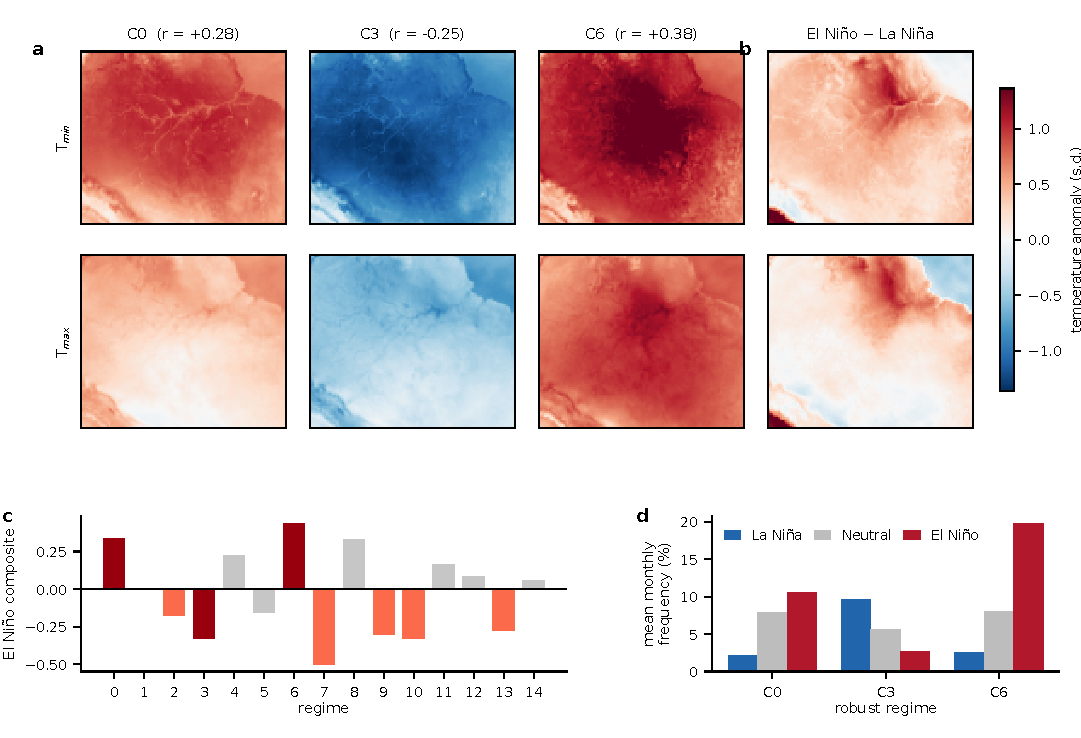
\includegraphics[width=\textwidth]{figures/fig4_physical.pdf}
\caption{\textbf{The robust regimes reproduce the ENSO fingerprint.}
\textbf{a}, Composite deseasonalised anomaly of the three FWER-significant regimes (columns; temporal ONI correlation in parentheses) for T$_{\min}$ (top) and T$_{\max}$ (bottom).
\textbf{b}, Model-independent ENSO fingerprint: mean anomaly of El Ni\~no months minus La Ni\~na months.
\textbf{c}, Centred spatial correlation of every regime composite with the El Ni\~no composite (colours as in Fig.~\ref{fig:enso_stats}); for every FWER-significant regime the sign matches the sign of its temporal ONI correlation (C6 $+0.44$, C0 $+0.34$, C3 $-0.33$).
\textbf{d}, Mean monthly occupancy of the robust regimes by ENSO phase: C6 fills 19.7\% of El Ni\~no months versus 2.5\% of La Ni\~na months; C3 shows the mirror-image preference.}
\label{fig:physical}
\end{figure}

\clearpage
\begin{appendices}

\section*{Extended Data}
\setcounter{figure}{0}
\renewcommand{\thefigure}{ED\arabic{figure}}

\begin{figure}[h]
\centering
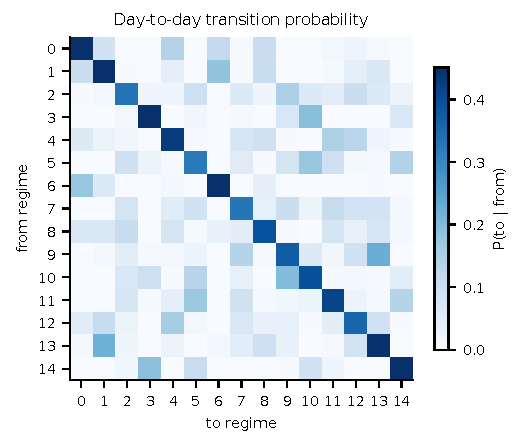
\includegraphics[width=.7\textwidth]{figures/ed1_transitions.pdf}
\caption{\textbf{Day-to-day regime transition matrix.} Transition probabilities concentrate on the diagonal (self-transitions), confirming that regimes are temporally coherent states rather than day-level noise.}
\label{fig:ed_transitions}
\end{figure}

\begin{figure}[h]
\centering
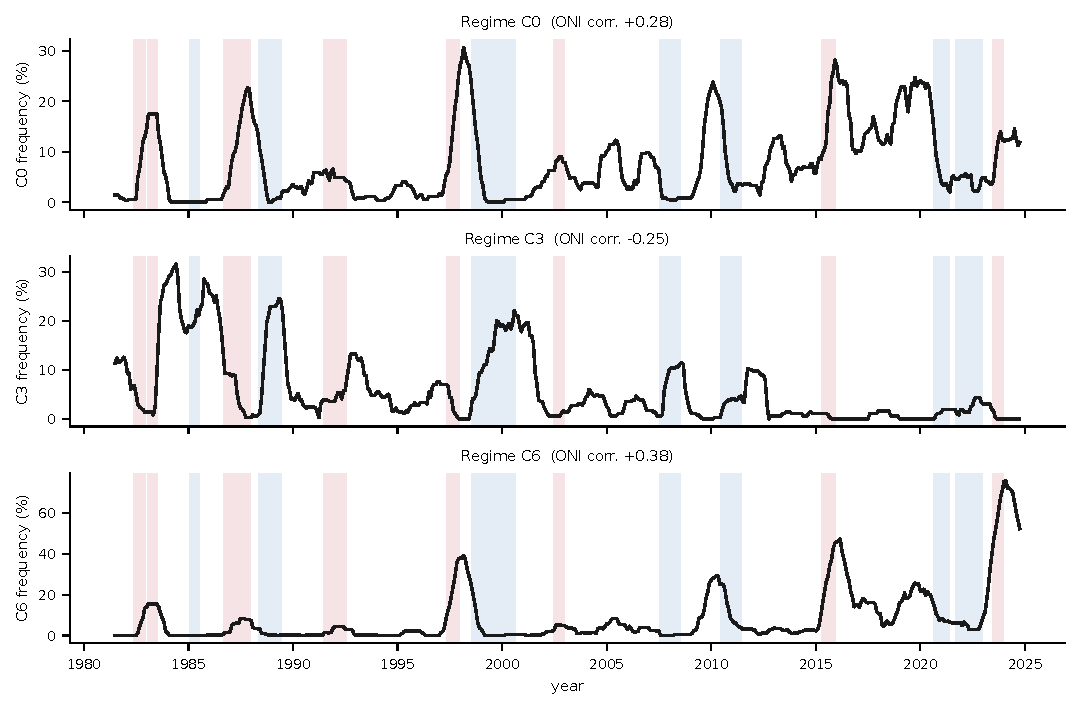
\includegraphics[width=\textwidth]{figures/ed2_timeseries.pdf}
\caption{\textbf{Occupancy of the robust regimes tracks ENSO through the record.} Twelve-month centred rolling occupancy of C0, C3 and C6; red (blue) shading marks El Ni\~no (La Ni\~na) months. The warm regimes C0 and C6 peak during major El Ni\~no events (1982/83, 1997/98, 2015/16, 2023/24) and are suppressed during La Ni\~na; C3 shows the opposite behaviour. The rising baseline of C6 and C0 and decline of C3 reflect the long-term trends of Fig.~\ref{fig:characterization}b.}
\label{fig:ed_timeseries}
\end{figure}

\begin{figure}[h]
\centering
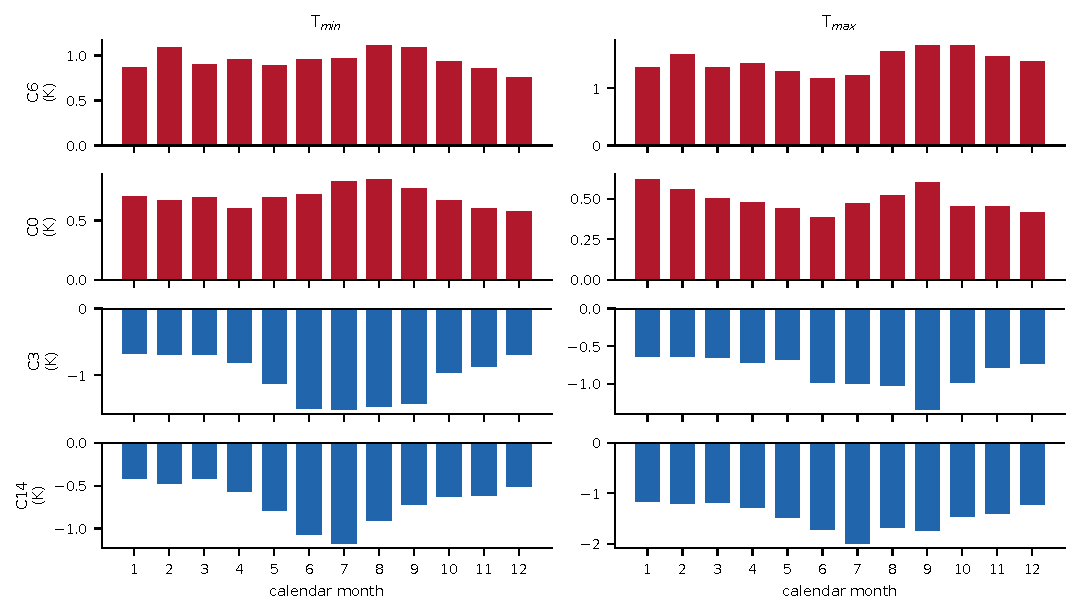
\includegraphics[width=\textwidth]{figures/ed3_sanity.pdf}
\caption{\textbf{Seasonally fair raw-temperature check, by calendar month.} Departure of domain-mean raw temperature from each calendar month's climatology for the two warmest (C6, C0) and two coolest (C3, C14) regimes, for T$_{\min}$ (left) and T$_{\max}$ (right). Warm (cool) regimes are warmer (cooler) than the monthly norm in every month of the year, ruling out seasonal aliasing.}
\label{fig:ed_sanity}
\end{figure}

\end{appendices}

\bibliography{refs}

\end{document}
